OpenGL is a 2D and 3D graphics API. It is a cross-platform API that specifies a standard for 3D graphics processing hardware. Android $1.0$ and later versions have support for \ac{opengles} $1.0$ and $1.1$ specifications. Android $2.2$ added support for \ac{opengles} $2.0$. \citep{androidopengl, khronosopengles}

\subsubsection*{Choice of \ac{opengles} Version}
When using \ac{opengles} on the Android platform, the default \ac{opengles} version is $1.x$. If you want to use version $2.0$ you need to explicitly write that you are using it. Version $2.0$ should have better performance and more possibilities than the older version, but the Android developers guide says:
\begin{quote}
\textit{"Developers who are new to OpenGL may find coding for \ac{opengles} 1.0/1.1 faster and more convenient."} \citep{androidopengl}
\end{quote}
Since we are beginners to OpenGL we have chosen version $1.x$. One big difference between $1.x$ and $2.0$ is that you have to write your own shaders in versions $2.0$, this allows for easier effects customization. The Train game does not really require much special effects other than simple drawing of textures.

\section{Design}

In this section we show how we use \ac{opengles} to draw on the screen. The design description gets very close to an implementation description, but a few specific methods will be described in more detail in the next section.

\subsection{Renderable Classes}

Considering the game and its purpose, we came up with different objects that should be rendered. \autoref{fig:renderables} shows a simplified version of the different objects/classes that can be rendered. We needed to draw texture at different positions on the screen and we needed to be able to move texture around on the screen. This is the general idea and based on this, the following classes were created.

\begin{figure}[H]
\centering
\includegraphics[page=2,width=1\linewidth]{img/opengl.pdf}
\caption{Class diagram of the objects that can be rendered.}
\label{fig:renderables}
\end{figure}

\begin{description}
\item[Coordination/Renderable:] In order to move objects around we have the abstract super class \lstinline|Coordination| which defines the methods to move. The abstract class \lstinline|Renderable| specifies that the objects needed to be rendered on the screen must implement the abstract methods: \lstinline|draw()|, \lstinline|getWidth()|, and \lstinline|getHeight()|. If some \lstinline|Renderable| object has to be be drawn more than once, then instead of making two identical \lstinline|Renderable| objects with different coordinates, we have a list of coordinates in \lstinline|Coordination|. The \lstinline|move| method will then move all the coordinates by the specified amount. It was also a possibility to move only one specific coordinate by the specified amount, but this last scenario was never needed.

\item[RenderableMatrix:] Since almost everything is moved relative to the train's speed we needed some kind of grouping of \lstinline|Renderable| objects, that were moved together. This is what \lstinline|RenderableMatrix| handles. It is possible to add other \lstinline|Renderable| objects to the \lstinline|RenderableMatrix|, this means that it is also possible to add matrices to\todo{To rendablesmatrices?} matrices. The \lstinline|addRenderMatrixItem()| method also has a color as parameter to use when drawing the \lstinline|Renderable|, this parameter is not shown on the figure to reduce the size of it. When calling \lstinline|draw()| on this class, it iterates through all \lstinline|matrixItems| and calls draw on them. The \lstinline|draw()| method's color parameter for the \lstinline|RenderableMatrix| is ignored, and instead it uses the color specified for each matrix item.

The \lstinline|RenderableMatrix| must also implement the abstract methods \lstinline|getWidth()| and \lstinline|getHeight()|. The width is calculated by the difference between the lowest x-coordinate to the greatest x-coordinate, and the same goes for the height with the y-coordinate instead. This feature was used at the time when this was designed, but has later become unnecessary.

The \lstinline|RenderableMatrix| is made with a new OpenGL matrix, this will be explained in more detail in \secref{sec:gamerendering}.

\item[Shape:] Everything that takes the form of a shape e.g. a square or a triangle, must inherit from the abstract class \lstinline|Shape|. All shapes consists of an array of vertices. The vertices for the \lstinline|Shape| determines how it is drawn relative to the coordinate.

Since we need wheels to rotate on the train, \lstinline|Shape| implements a method to rotate the \lstinline|Shape| around its center.

\item[Square:] The \lstinline|Square| is initialised with a size in the constructor, and then vertices are created according to the specified size. We decided that the \lstinline|Square| should be drawn from the top-left corner on its coordinates.

The color in the \lstinline|draw()| method's parameter specify the color of the square.

\item[GradientSquare:] This is similar to the \lstinline|Square|, instead this square is initialised with two colors to create either a horizontal or a vertical color gradient between the two colors.

\item[Texture:] This is the most important and most used class when creating our game. Since all pictures/images are 'square', it inherits from \lstinline|Square|, and then the texture is mapped onto that \lstinline|Square|.

This class must at some point load a resource pointer to a texture pointer. The loaded texture will always stretch to the size of the \lstinline|Square| that it is drawn upon. The \lstinline|Texture| class also implements ways to keep the original aspect ratio of the texture. Although not shown in the figure, the \lstinline|loadTexture()| method also has an aspect ratio option that allows the size of the \lstinline|Square|, containing the texture, to resize based on the size of the texture.

During loading of a piece of texture, the texture is converted to a \ac{pot} sized texture, \secref{sec:potsupport} explains why. \ac{opengles} has maximum dimensions for texture which is dependent on the device in use \citep{glutils}. Each piece of texture is checked whether they respect the maximum dimensions, if it does not it is scaled down.

The \lstinline|draw()| method must be overridden in order to draw the loaded texture. In this case it is possible to change the color that the \lstinline|Texture| is drawn with. No matter what color the original \lstinline|Texture| is, a color filter can be put on top of that on each call of the draw method.

\item[Text:] Adds the possibility to draw text. \lstinline|loadText()| generates a bitmap with the specified text to use as texture. This is an easy way to draw text, but if you need to draw text that changes all the time, then \lstinline|loadText()| is a slow way to do it. Fortunately we only need to load one time for each \lstinline|Text| object.

\item[GlPictogram:] Adds the possibility to draw a pictogram. The method \lstinline|loadPictogram()| generates a bitmap of the pictogram image, and then uses it as the texture for the object. To draw the pictogram text, a \lstinline|Text| object is used.
\end{description}

\subsection{Texture Power-of-two Support}\label{sec:potsupport}
Some \ac{opengles} devices does not support texture with a \ac{npot} size, they only accept texture with a \ac{pot} size, i.e. $2^x$. Android developers reference states that you should perform a check whether the current context supports \ac{npot}. \citep{glutils}

You get an increase of performance when using \ac{pot}, and at the time when the first version of OpenGL was created, the hardware needed this extra performance. Years later hardware only gained an insignificant increase of performance so they allowed \ac{npot}. Some embedded systems using \ac{opengles} still gain a significant increase in performance, and this is why some devices require texture to be \ac{pot}. (We were not able to find official citation, the best we could find is this \citep{potperformance})

Instead of performing a check to see whether the current context supports \ac{npot}, we choose to always use \ac{pot}. Even if it is not necessary it will still give a small performance increase. The way we achieve this is to still use texture with a \ac{npot} size, convert the texture to \ac{pot} size, and then stretch it relative to the change in size. However this will also consume a lot more memory, but the train game does not require that much memory even with \ac{pot} sized texture.
\begin{figure}[H]
\begin{minipage}[b]{0.5\columnwidth}
\centering
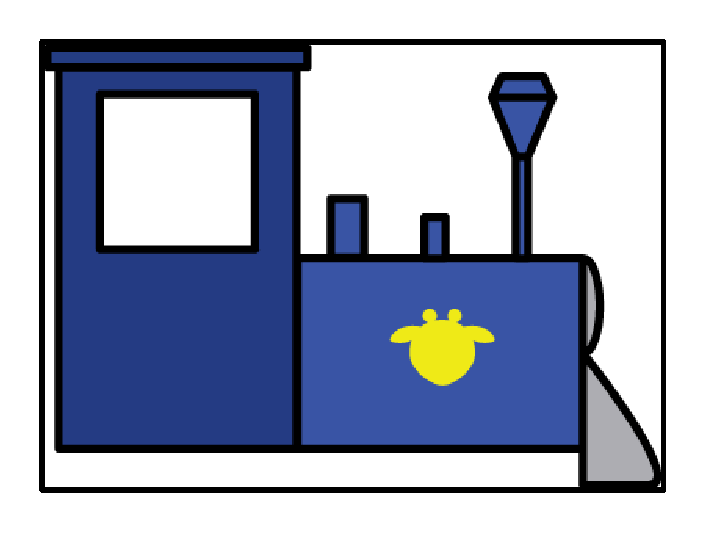
\includegraphics[page=1,width=0.8\columnwidth]{img/powerOfTwo.pdf}
\caption{The \ac{npot} train texture inside the \lstinline|Square| container.\label{fig:train}}
\end{minipage}
\hspace{0.5cm}
\begin{minipage}[b]{0.5\columnwidth}
\centering
\includegraphics[page=2,width=0.8\columnwidth]{img/powerOfTwo.pdf}
\caption{The \ac{pot} train texture.\label{fig:trainpot}}
\end{minipage}
\end{figure}
\autoref{fig:train} shows the train texture inside the \lstinline|Square| container. The black line illustrates the \lstinline|Square|, this is shown for the sake of the example and it is of course not shown in the actual application. The texture has a size of $396 \times 284$ pixels, and need to be converted to a \ac{pot} size.

\autoref{fig:trainpot} shows the train texture with alpha channels to the right and below the texture to obtain a \ac{pot} texture with the size of $512 \times 512$ pixels.
\begin{figure}[H]
\begin{minipage}[b]{0.5\columnwidth}
\centering
\includegraphics[page=3,width=0.8\columnwidth]{img/powerOfTwo.pdf}
\caption{The \ac{pot} train texture inside the \lstinline|Square| container.\label{fig:trainneedcrop}}
\end{minipage}
\hspace{0.5cm}
\begin{minipage}[b]{0.5\columnwidth}
\centering
\includegraphics[page=4,width=0.8\columnwidth]{img/powerOfTwo.pdf}
\caption{The \ac{pot} train texture after stretching.\label{fig:trainresult}}
\end{minipage}
\end{figure}
When we take the new \ac{pot} sized texture and insert it into the \lstinline|Square| the texture will still clamp to the edges. \autoref{fig:trainneedcrop} shows the clamped train texture.

We need to adjust the texture in order to fit the \ac{pot} texture inside the \lstinline|Square|. We stretch the texture by mapping the texture outside of the \lstinline|Square| relative to the change in size from \ac{npot} to \ac{pot}. Since nothing outside the borders of the \lstinline|Square| is drawn, then you could also say that the extra alpha channels are cropped away. \autoref{fig:trainresult} shows the result of the texture conversion from \ac{npot} to \ac{pot}.

\subsection{Game Rendering}\label{sec:gamerendering}

To draw the game we are using an \lstinline|android.opengl.GLSurfaceView|. To draw on the \lstinline|GLSurfaceView| we are required to make our own class which implements \lstinline|android.opengl.GLSurfaceView.Renderer| \citep{androidopengl}. \autoref{fig:game} shows a simplified version of the different objects/classes that draws the game.

\begin{figure}[H]
\centering
\includegraphics[page=3,width=1\linewidth]{img/opengl.pdf}
\caption{Class diagram of the objects involved with drawing the game.}
\label{fig:game}
\end{figure}

\begin{description}

\item[GlRenderer] This is our implementation of a \lstinline|Renderer|, the class must override \lstinline|onDrawFrame()|, \lstinline|onSurfaceChanged()|, and \lstinline|onSurfaceCreated()|. These three methods are all run on a thread that is automatically created for us when we implement the \lstinline|Renderer|. \todo{fix inline} When the \lstinline|Renderer| is started, it runs the method \lstinline|onSurfaceCreated()|. This is where we initialize the \lstinline|GameDrawer| object. After the surface is created it runs \lstinline|onSurfaceChanged()|, it is at this time the \lstinline|Renderer| knows how big the surface is in pixels. We use this information to load all the texture in the game, by calling \lstinline|loadGame()| in the \lstinline|GameDrawer|. When the game is loaded it runs \lstinline|onDrawFrame()| continuously, where we draw the game by calling \lstinline|drawGame()| in the \lstinline|GameDrawer|.

Even though the game is in \ac{2d} we choose to create it in a \ac{3d} environment. When \lstinline|onSurfaceChanged| runs we create our main \ac{3d} matrix. \ac{opengles} $1.x$ maintains a stack of matrices, the stack is required to contain at least one matrix. It will give an error if you pop all matrices. The \lstinline|RenderableMatrix| is drawn by translating its coordinates, and then pushing a new matrix on the stack, then this new matrix on the stack can be translated around in\todo{Around in?} and draw our \lstinline|Renderable| objects. When a matrix is popped from the stack you return to the same position as when you pushed a new matrix.\citep{openglspecs}

\item[GameDrawer] When this object is initialized it creates all the \lstinline|GameDrawable| objects, and add them to a list in the order they should be drawn. When the \lstinline|GlRenderer| calls \lstinline|loadGame()| or \lstinline|drawGame()|, the \lstinline|GameDrawer| simply iterates through the list of \lstinline|GameDrawable| objects, and calls \lstinline|load()| or \lstinline|draw()| on them. Loading will only happen each time the surface is changed, i.e. when the activity is created.

An important thing the \lstinline|GameDrawer| does, although not shown in the figure, is maintaining the current position in the frustum. \lstinline|translateTo()| will translate the current position to the specified coordinate. \lstinline|RenderableMatrix| also maintains the position of the matrix that it is working with. \lstinline|GameDrawer| and \lstinline|RenderableMatrix| is actually pretty much the same, the main difference is that \lstinline|GameDrawer| draws \lstinline|GameDrawable| objects and \lstinline|RenderableMatrix| draws \lstinline|Renderable| objects. It would be an elegant solution to refactor the code to get rid of either \lstinline|RenderableMatrix| or \lstinline|GameDrawer| instead, but we deem that we want to use both classes in order to separate the main \ac{3d} matrix from the others.

\item[GameDrawable] This is an abstract class. Classes inheriting from this must implement \lstinline|load()| and \lstinline|draw()|. In the \lstinline|load()| method, drawables should add coordinates to \lstinline|Renderable| objects, and call their respective load methods. In the \lstinline|draw()| method, it should call the \lstinline|Renderable| objects respective \lstinline|draw()| methods, or use either \lstinline|translateAndDraw()| or \lstinline|translateRotateAndDraw()|. The two 'translate' methods both translate to a coordinate, by using \lstinline|translateTo()| in the \lstinline|GameDrawer|, and then draw the \lstinline|Renderable|. Note that \lstinline|translateRotateAndDraw()| will only rotate \lstinline|Shape| objects. We do not allow rotation of \lstinline|RenderableMatrix|.

\item[GameData] When the activity is created then we create one \lstinline|GameData| object. This contains all the data needed to determine what has happened, what is happing, and what will happen later. When the object is initialized it will set the \lstinline|numberOfStations| attribute according to the current game configuration.

\lstinline|pixelMovement| is the number of pixels that the train has moved in the current frame. It is based on the \lstinline|currentTrainVelocity| and the \lstinline|timeDifference| between this frame and the last one. \lstinline|numberOfStops| is how many times the train has stopped in this game session, and it is also used as an index in the \lstinline|nextStoppingPosition| array which is an array with all the locations where the train should stop. The stopping positions are based on \lstinline|totalDistanceTraveled| which is the total number of pixels the train has moved. Of all the attributes, it is only \lstinline|pixelMovement| that is private. Some of the other attributes should also have protected access, but in this case it is better looking to access attributes directly instead of using get methods all the time.

The \lstinline|GameDrawer| starts its \lstinline|drawGame()| method by calling \lstinline|updateData()| which updates the above attributes. It also checks whether the train should begin deceleration based on the method \lstinline|brakingDistance()| and the stopping positions. In order to get the train started or stopped the method \lstinline|accelerateTrain()| and \lstinline|decelerateTrain()| are used. They set a flag that indicates the train is changing velocity and then set a positive or negative acceleration constant. \lstinline|performAcceleration()| updates the train's velocity and makes sure that the train gets a nice smooth stop/start.

Do not mistake the method \lstinline|getTotalTravelDistance()| and the attribute \lstinline|totalDistanceTraveled| with each other. The method returns the total distance the train must travel for this game session plus the width of the screen, this is used to generate all of the background for the game session.

\lstinline|onPause()| sets a flag indicating that the game is paused, it then saves the train's velocity and sets it to 0. The \lstinline|GameDrawable| objects then know that the game is paused and can stop updating their position. \lstinline|onResume| will restore the train's velocity and the game continues.

\end{description}

\subsection{Frustum}\label{sec:frustum}

When our renderer is created it sets up \ac{3d} perspective. \autoref{fig:clippingplane} shows a perspective looking at the frustum between the near and far clipping planes.
\begin{figure}[H]
\centering
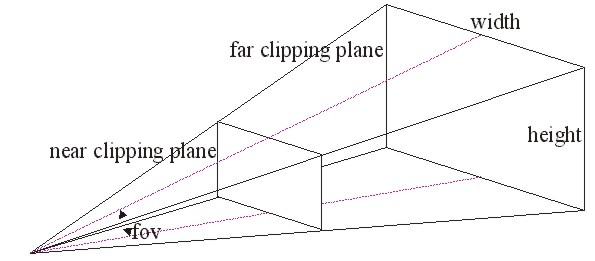
\includegraphics[width=0.9\linewidth]{img/clippingplane.jpg}
\caption{Perspective (Figure from \citep{clippingplane}).}
\label{fig:clippingplane}
\end{figure}
Inside the frustum is where you should draw, if you try to draw outside the bounds of the frustum, then nothing will be drawn and it will not consume resources. When setting up the game perspective we provide \ac{opengles} with the current aspect ratio of the screen, a field of view angle (denoted 'fov' in \autoref{fig:clippingplane}), and the depth of the near and far clipping planes. The width and height increases in size when we go deeper into the perspective, but the field of view angle always spans relative to the height of the screen. The width is always relative to the aspect ratio. This means that if we draw a square at a specific coordinate in the perspective, then the square will always have the same percent of space above and below it on the screen, but the space to the right and to the left of the square changes according to the aspect ratio of the screen.

The coordinate $(0, 0, 0)$ is where the perspective starts, or you could say it is where we are looking from. If you translate into the depth of the frustum e.g. $(0, 0, 50)$, then you are at the center of the perspective/screen.

The tablet has a resolution of $1280 \times 800$, but since it always displays a system bar with back-button, notifications, etc. we only have $1280 \times 752$ pixels of the screen available. All the graphics created for the game was made on a canvas with the same size as what we have available. In order to draw the graphics on the tablet screen we have to find the depth where the width and height in the frustum are the same as our screen size $1280 \times 752$.
\begin{figure}[H]
\centering
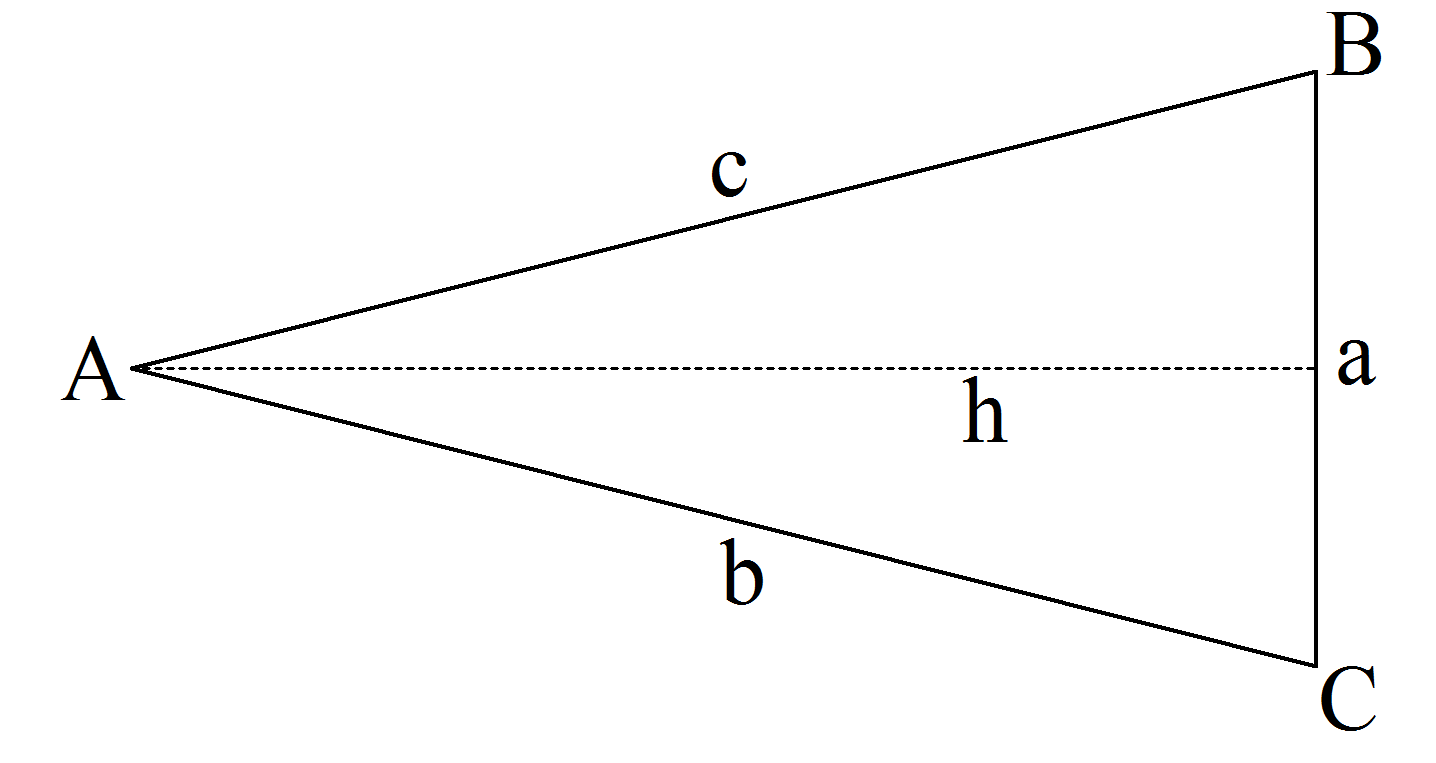
\includegraphics[width=0.5\linewidth]{img/trekant.png}
\caption{Perspective seen from the side.}
\label{fig:frustumside}
\end{figure}
\autoref{fig:frustumside} shows the perspective seen from the side, we want to find the height $h$ (depth) of the triangle when $a$ is the same size as our tablet $a = 752$. We have chosen a field of view angle to be $A = 45^{\circ}$. Since the angles $B$ and $C$ are the same size then
$$B = C = \frac{180^{\circ} - A}{2} = 67.5^{\circ}$$
Given $a$ and all the angles of the triangle, then $h$ is given by
$$h = \frac{a}{2} \times tan(B) = 907.7442$$
Now we have the depth of the perspective where one pixels of a texture corresponds to one pixels on the tablet screen. This will also make it possible to use pixels per millisecond as an actual unit of speed for our game.